\chapter{Proposta de Trabalho}\label{chap:proposta}

\section{Motivação e Objetivo}

% Motivação Tema
No Capítulo~\ref{chap:revisao} foram apresentados os
métodos que buscam modificar os conjuntos de dados para 
torná-los mais representativos para o problema em estudo. 
Discutiu-se que os métodos automáticos impedem que os
usuários orientem essas modificações e ao mesmo tempo
imponham seus conhecimentos sobre os resultados. 
Buscando tratar este problema apresentou-se as ferramentas 
visuais que surgem como uma interessante alternativa
por permitirem a interação dos usuários, mas que ainda
apresentam certas limitações em relação às interfaces
utilizadas e  aos mecanismos de interação propostos.

O uso de ferramentas visuais como alternativa aos métodos
automáticos não é exclusivo aos trabalhos relacionados
ao aqui proposto. Na verdade, toda a área de
Mineração Visual de Dados~\cite{Wong1999} (MVD),
\emph{Visual Data Mining}, tem como objetivo justamente
envolver os usuários em tarefas que até em tão eram
executadas de maneira totalmente automática. A principal
motivação desta área parte do princípio de quando o usuário
consegue compreender o resultado apresentado por uma
representação visual, então ele confia neste resultado e
consegue tirar melhor proveito das análises.

Uma característica fundamental para essas ferramentas é manter a
simplicidade em todos aspectos do sistema. No entanto, foi
visto no Capítulo~\ref{chap:revisao} que muitas das
ferramentas propostas se baseiam em interfaces
demasiadamente complexas, as quais exigem do usuário um
certo período de treinamento para um uso efetivo. Tendo em
vista que o objetivo das ferramentas visuais é tornar as
análises mais intuitivas, qualquer tipo de obstáculo, como
a necessidade de treinamento do usuário, pode ser
desfavorável ao se comparar com os métodos automáticos.

Um outro aspecto que deve ser levado em consideração para o
desenvolvimento dessas ferramentas é permitir seu uso em
diversos domínios. Mas para isso, diferentes mecanismos de
interação devem ser oferecidos, já que nenhum mecanismo
será capaz de operar otimamente para todas as aplicações.
No capítulo anterior foi discutido que nenhuma
das ferramentas apresentadas consegue unir em um único
ambiente os principais mecanismos necessários para a
modificação efetiva de conjuntos de dados.

% Falar da questão de características em subconjuntos de
% dados e a necessidade de se interagir com itens.

Deste modo, o objetivo deste trabalho de mestrado pode ser
declarado da seguinte maneira:

\begin{quote}
    \emph{``Este projeto de mestrado tem como objetivo
        desenvolver uma ferramenta visual interativa que
        permita aos usuários modificarem conjuntos de dados
        para torná-los mais representativos. As modificações
        serão realizadas a partir de três principais
        mecanismos de interação: seleção, construção e
        transformação de atributos. Com dados melhor
        representados, os métodos que operam sobre eles,
        como classificadores e agrupadores de dados, devem
        apresentar melhores resultados. Será por meio de uma
        quantificação dessa melhoria que será feita a
    validação da nova ferramenta desenvolvida.''}
\end{quote}

A seguir apresenta-se a metodologia proposta para o
desenvolvimento de cada um desses mecanismos e da ferramenta como um todo.

\section{Metodologia}

A metodologia proposta por este trabalho é ilustrada pela Figura~\ref{fig:met}. O processo inicia pelo cálculo da similaridade entre as dimensões. Com base neste cálculo, cria-se uma matriz de distâncias entre os atributos que é utilizada para projetá-los em um espaço bidimensional.   

inicia pela escolha de uma medida para o cálculo da similaridade entre pares de dimensões. Com base nessas distâncias projeta-se as dimensões utilizando alguma técnica de projeção multidimensional, como MTS. Neste ponto permite-se que o usuário utilize os mecanismos interativos de redução de dimensionalidade e de transformação do espaço de atributos. Ele pode, por exemplo, construir um espaço dimensional reduzido que é prontamente apresentado em visualizações coordenadas. Finalmente, se o resultado obtido não for satisfatório, o usuário pode iniciar novamente o ciclo partindo do novo espaço dimensional construído, ou pode realizar novas manipulações sobre os dados.

% Melhorar este parágrafo e colocar uma figura para ilustrar o processo.

\begin{figure}[h!]
    \centering
    \begin{subfigure}[b]{0.5\textwidth}
        \centering
        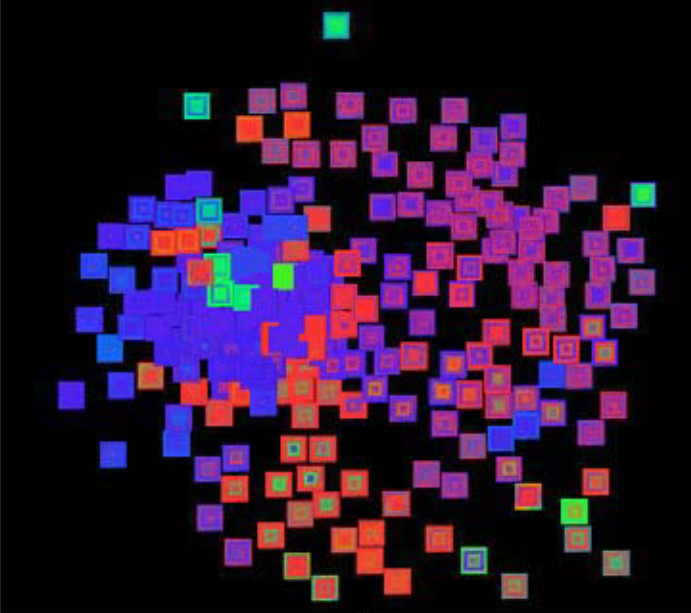
\includegraphics[width=\textwidth]{images/var1.png}
        \caption{}
        \label{fig:var1}
    \end{subfigure}%
    ~ %add desired spacing between images, e. g. ~, \quad, \quad etc.
    \begin{subfigure}[b]{0.475\textwidth}
        \centering
        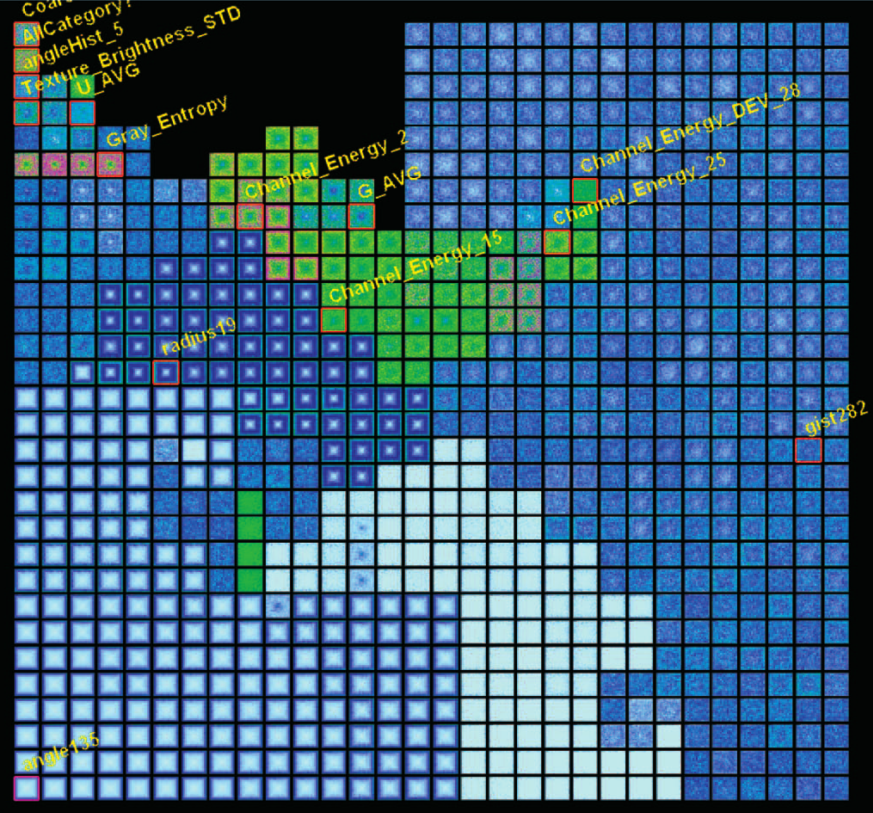
\includegraphics[width=\textwidth]{images/var2.png}
        \caption{}
        \label{fig:var2}
    \end{subfigure}
    \caption[VaR: Value and Relation]{acid}
    \label{fig:met}
\end{figure}


\subsection{Similaridade entre Dimensões}\label{ss:sim}

Uma tarefa fundamental para a execução deste trabalho é maneira como define-se a            similaridade entre as dimensões. Este problema pode ser formulado da seguinte maneira~\cite{Ankerst1998}: Dado um conjunto de dados contendo $n$ elementos com $m-$dimensões, suas colunas podem ser descritas por $m$ vetores $A_i~(0 \leq i < m)$, cada uma contendo $n$ números reais $a_{i,k}, (0 \leq k < n)$. Deseja-se definir uma medida de similaridade $S$ que dado dois vetores retorne um número real ($S : \mathbb{R}^n \times \mathbb{R}^n \rightarrow \mathbb{R}$) que satisfaça as seguintes propriedades:

\begin{enumerate}

    \item Positividade: $\forall A_i,A_j \in \mathbb{R}^n: S(A_i,A_j) \geq 0 $

    \item Reflexividade: $\forall A_i,A_j \in \mathbb{R}^n: (A_i = A_j) \Leftrightarrow S(A_i,A_j) = 0 $

    \item Simetria: $\forall A_i,A_j \in \mathbb{R}^n: S(A_i,A_j) = S(A_j,A_i)$, onde $(0 \leq i,j < d)$.

\end{enumerate}

Uma medida de similaridade entre duas variáveis $x$ e $y$ muito utilizada é o coeficiente de correlação linear de Pearson $p$, dado por:

\begin{equation}
    p(x,y) = \frac{cov(x,y)}{\sqrt{var(x)var(y)}},
\end{equation}

\noindent onde $var$ corresponde à variância e $cov$ à covariância. Quando $x$ e $y$ são completamente dependentes entre si, o valor de $p(x,y)$ é $1$ ou $-1$. Caso não exista nenhuma dependência linear entre as variáveis, o valor obtido é $0$. Porém, nos conjuntos de dados as relações entre as variáveis nem sempre são lineares e daí que surge a maior limitação deste coeficiente. Como pode ser observado pela Figura~\ref{fig:corrs} e pelos valores apresentados na Tabela~\ref{tab:corrs}, a medida não é capaz de capturar dependências não lineares entre as variáveis. 

\begin{figure}[h!]
    \centering
    \begin{subfigure}[b]{0.5\textwidth}
        \centering
        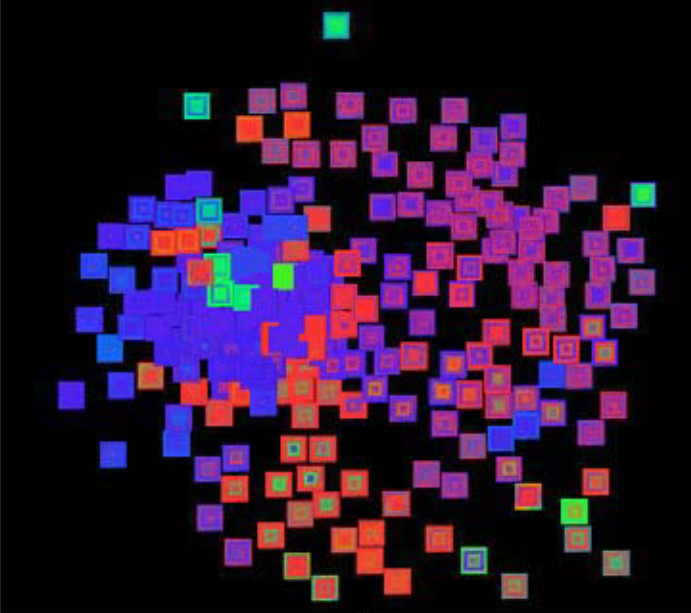
\includegraphics[width=\textwidth]{images/var1.png}
        \caption{}
        \label{fig:var1}
    \end{subfigure}%
    ~ %add desired spacing between images, e. g. ~, \quad, \quad etc.
    \begin{subfigure}[b]{0.475\textwidth}
        \centering
        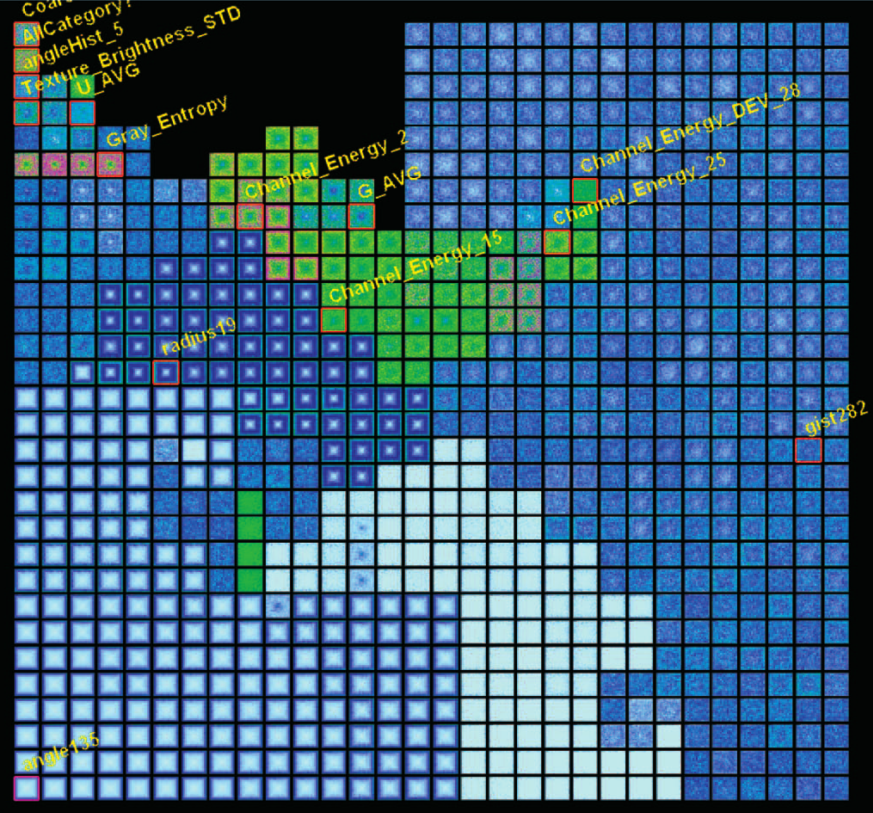
\includegraphics[width=\textwidth]{images/var2.png}
        \caption{}
        \label{fig:var2}
    \end{subfigure}
    \caption[VaR: Value and Relation]{acid}
    \label{fig:corrs}
\end{figure}

\begin{table}
    \caption[Cronograma de atividades]{Cronograma de Atividades. As marcações em preto        indicam atividades que são priorizadas no período.}
    \begin{center}
        \begin{tabular}{|c|c|c|c|c|c|c|}
        \end{tabular}
    \end{center}
    \label{tab:corrs}
\end{table}

% Falar de discretização? (Parzen windows, Torkkola, 2003)

% Introduzo MI (ler Kraskov) 

% Descrevo um estimador de MI, outros estimadores de MI: 12,13,14

% Apresento o problema de MI e MIC como a solução (apresentar complexidade computacional da MIC)

Na literatura encontram-se diversos outros métodos que poderiam ser utilizados para o cálculo de similaridade. Métodos de regressão~\cite{Friedman2001, Cleveland1988, Stone1977} têm bom desempenho quando as relações podem ser descritas por uma função, mas além desta situação falham em encontrar até os mais simples relacionamentos. Os métodos baseados em curvas principais~\cite{Hastie1989, Tibshirani1992, Delicado2008} e outros de correlação~\cite{Reny1959, Breiman1985, Kosorok2009} são aplicáveis a um domínio mais abrangente de dados, porém não conseguem capturar os relacionamentos tão eficientemente quanto a medida MIC~\cite{Reshef2011} mesmo para casos simples, como pode ser observado pela Tabela~\ref{tab:corrs}.    

A qualidade de uma medida de similaridade costuma variar de acordo com o domínio em que é aplicada. Normalmente, uma medida é dita adequada quando há uma concordância entre o valor obtido e a opinião de um especialista da área. No entanto, mesmo um especialista sobre um assunto pode ter dificuldade em determinar com precisão a semelhança entre dois objetos. Assim, é muito difícil definir um modelo matemático que meça a similaridade entre dois atributos com precisão para todas as aplicações de forma genérica. A MIC é uma medida que se propõe a executar esta difícil tarefa e por isso foi escolhida como a medida de similaridade entre dimensões a ser utilizada neste trabalho. 

\subsection{Mapeamento dos Itens no Espaço Bidimensional}
\subsection{Mapeamento das Dimensões no Espaço Bidimensional}
\subsection{Mapeamento no Espaço Bidimensional}

O mapeamento dos elementos em um espaço bidimensional se baseia em algum método de redução de dimensionalidade. 

Um ponto fundamental para o mapeamento dos elementos no plano é compreender o erro embutido no processo. O resultado ótimo de qualquer método de redução é levar os dados de m em p, onde p equivale à dimensionalidade intrínseca dos dados. No entanto,  não há garantias de que p equivale à um espaço bidimensional, assim ao mapear os dados em um plano, a dimensionalidade dos dados será reduzida além da dimensionalidade intrínseca e consequentemente haverá perda de informação.

Conclui-se que independentemente do método de redução adotado, a não ser que a dimensionalidade intrínseca dos dados seja equivalente a dois, haverá um erro ao mapear os dados em um plano. Dois tipos de erros podem ocorrer: pontos similares posicionados distantes entre si (falsos negativos), ou pontos diferentes posicionados próximos entre si (falsos positivos). 

Em uma analogia à tarefa de recuperação de informação \emph{information retrieval}, esses erros podem ser associados respectivamente às medidas de precisão \emph{precision} e revocação \emph{recall} (citar 8 e 9 de Kasai).

% Tenho que falar do erro embutido 
Uma vez definido o cálculo de similaridade entre as dimensões, cria-se uma matriz de distâncias 

Não é possível ter garantias de que a dimensionalidade intrínseca dos dados se encaixa no plano bi
Ao mapear os dados em um plano bidimensional não é possível garantir que a dimensionalidade  

\subsection{Projeção das Dimensões}

\subsection{Projeção dos Itens}

O propósito principal da visualização da projeção dos itens é possibilitar que o usuário crie subconjuntos dos dados, por exemplo, possibilitar a remoção de \emph{outliers} ou a inspeção de um grupo de interesse.

Além disso esta visualização serve como um ferramenta adicional aos resultados dos classificadores para avaliar a separação entre os itens.


%--------------------------------------------------------------------------------
\subsection{Mecanismos de Interação}

\subsubsection{Seleção de Atributos}

Em tarefas de seleção de característica basicamente deseja-se solucionar basicamente dois problemas. 
O primeiro, chamado de mínimo ótimo (\emph{minimal optimal})~\cite{Kohavi1997}, consiste em construir um subconjunto dos atributos de entrada evitando ao máximo a redundância entre eles. 
Um caso prático deste problema trata-se da construção de um classificador, onde ao se evitar redundância entre os atributos de entrada pode fazer com que o método obtenha ganhos tanto no tempo de execução quanto na qualidade dos resultados obtidos. 
Já o segundo, conhecido como todos relevantes (\emph{all relevant})~\cite{Nilsson2007}, equivale a encontrar todos os atributos que são de algum modo relevantes para a compreensão do fenómeno observado. 
Uma aplicação real deste segundo problema pode ser encontrada no contexto de análise de expressões gênicas, onde pode-se, por exemplo, identificar quais genes apresentam maior relação com o diagnóstico de alguma doença. 

O mecanismo de seleção aqui proposto viabiliza trabalhar sobre esses dois problemas.

\subsubsection{Combinação de Atributos}

O resultado obtido pela combinação deve ser melhor do que a de seleção, porém é também menos intuitivo ao usuário. Mas de qualquer modo a abordagem é melhor aplicar PAC em todo o conjunto de dados (tirei isso de CHOR, se precisar citar: pelo o que pode ser observado no levantamento bibliográfico os métodos de combinação tendem a oferecer melhores resultados, no entanto...).  

\subsection{Forma de Avaliação}

% Tenho que falar aqui que vou aplicar diferentes métodos de redução (eventualmente ter que explicar os que eu escolhi cada um, de preferência falar que cada um tem uma característica específica) e em seguida vou verificar a qualidade da classificação e o tempo de execução do classificador.

Vou comparar com outros métodos de redução.

Em alguns trabalhos~\cite{Joshi2007} a comparação é feita sobre a taxa de acertos da classificação com os dados originais e com os dados reduzidos com a técnica proposta. No entanto, esta validação pode ser questionada, pois desconsidera a influencia que outras técnicas de redução poderiam ter nos resultados.

Para se comprar com seleção de características, \cite{Guyon2003} diz para usar um classificador linear (linear SBM) e selecionar as variáveis de duas maneiras: por meio de um ranking a partir do coeficiente de correlação ou informação mútua; ou pelo uso de um método de forward (ou backward) selection.

\cite{Medeiros2011} apresenta três índices para se comparar diferentes técnicas de redução. Aponta que devido a heterogeneidade dos métodos, certas convenções devem ser estabelecidas para se obter uma comparação justa.

A forma mais adotada na literatura para a avaliação de métodos de redução de dimensionalidade é a comparação dos erros obtidos em tarefas de classificação ao utilizar diferentes técnicas. 

Ao reduzir o número de atributos irrelevantes ou redundantes, pode-se melhorar o desempenho computacional e a precisão das técnicas operando sobre os dados, como agrupadores e classificadores de dados. Pretende-se avaliar as contribuições deste trabalho justamente pela quantificação do desempenho de tais métodos ao utilizar as técnicas desenvolvidas, seguida de uma comparação com técnicas já estabelecidas na literatura.

% O popular método K Means será utilizado neste trabalho para se avaliar Para se avaliar o resultado obtido por agrupadores de dados, frequentemente utiliza-se a medida da silhueta e o índice I. A silhueta mede a .... O índice I é utilizado para...

% Falo de Sam Precisão, Recall (FAN?) e sei la o que...


%--------------------------------------------------------------------------------
\section{Resultados Esperados}

\section{Resultados Preliminares}

\section{Plano de Atividades e Cronograma Previsto}\label{sec:cronograma}

As principais atividades deste trabalho de mestrado são as seguintes:

\begin{enumerate}

    \item Cumprimento dos créditos das disciplinas exigidos pelo programa;

    \item Exame de proficiência em língua inglesa;

    \item Levantamento bibliográfico sobre técnicas de visualização computacional e redução de dimensionalidade;   

    \item Levantamento bibliográfico sobre técnicas visuais interativas para redução de dimensionalidade;  

    \item Adoção e implementação de uma metodologia para o cálculo da similaridade entre dimensões;

    \item Escrita da monografia de qualificação e sua apresentação para uma banca avaliadora;

    \item Implementação de um modelo visual que transmita simultaneamente informações sobre os itens e dimensões de uma base de dados;

    \item Desenvolvimento de mecanismos de seleção e combinação para redução interativa de dimensionalidade;

    \item Desenvolvimento de um mecanismo interativo para transformação do espaço de atributos;

    \item Avaliação dos Resultados;

    \item Redação de artigos científicos e participação em congressos e eventos; 

    \item Escrita da dissertação de mestrado bem como sua apresentação para uma banca avaliadora;

\end{enumerate}

O cronograma de execução das atividades é apresentado na Tabela~\ref{t:atividades}, assumindo um projeto de duração de vinte e quatro meses.

\newcommand{\y}{\color{black}\rule{20pt}{7pt}}
\newcommand{\x}{\hspace*{20pt}}
\renewcommand{\r}{\color{cinza}\rule{20pt}{7pt}}

\setlength{\tabcolsep}{0pt}

\begin{table} 
    \caption[Cronograma de atividades]{Cronograma de Atividades. As marcações em preto indicam atividades que são priorizadas no período.}
    \begin{center}
        \begin{tabular}{|c|c|c|c|c|c|c|}
            \cline{2-7}
            \multicolumn{1}{l|}{} & \multicolumn{2}{c|}{2012} & \multicolumn{2}{c|}{2013} &        \multicolumn{2}{c|}{2014} \\
            \hline \ Atividade\ \ 
            & 1\textordmasculine\ S. & 2\textordmasculine\ S. 
            & 1\textordmasculine\ S. & 2\textordmasculine\ S. 
            & 1\textordmasculine\ S. & 2\textordmasculine\ S. \\
            \hline \hline                                        
            %     &       2012        &       2013         &       2014       \\
            1     &\y\y    &\y\y      &\x\x     &\x\x      &\x\x     &\x\x    \\ \hline
            2     &\x\y    &\x\x      &\x\x     &\x\x      &\x\x     &\x\x    \\ \hline
            3     &\x\x    &\y\y      &\y\y     &\r\r      &\r\r     &\x\x    \\ \hline
            4     &\x\x    &\y\y      &\y\y     &\r\r      &\r\r     &\x\x    \\ \hline
            5     &\x\x    &\x\x      &\y\y     &\x\x      &\x\x     &\x\x    \\ \hline
            6     &\x\x    &\x\x      &\y\y     &\x\x      &\x\x     &\x\x    \\ \hline
            7     &\x\x    &\x\x      &\x\y     &\r\x      &\x\x     &\x\x    \\ \hline
            8     &\x\x    &\x\x      &\x\x     &\r\r      &\x\x     &\x\x    \\ \hline
            9     &\x\x    &\x\x      &\x\x     &\r\r      &\x\x     &\x\x    \\ \hline
            10     &\x\x    &\x\x      &\x\x     &\x\r      &\r\r     &\x\x    \\ \hline
            11     &\x\x    &\x\y      &\y\y     &\r\r      &\r\r     &\x\x    \\ \hline
            12     &\x\x    &\x\x      &\x\x     &\x\r      &\r\r     &\x\x    \\ \hline
            %     &       2012        &       2013         &       2014       \\
        \end{tabular}
    \end{center}
    \label{t:atividades}
\end{table}
